\documentclass[tikz, margin = 2pt]{standalone}    
\usepackage{tikz}  
\usetikzlibrary{decorations.pathreplacing,calligraphy}
\begin{document}
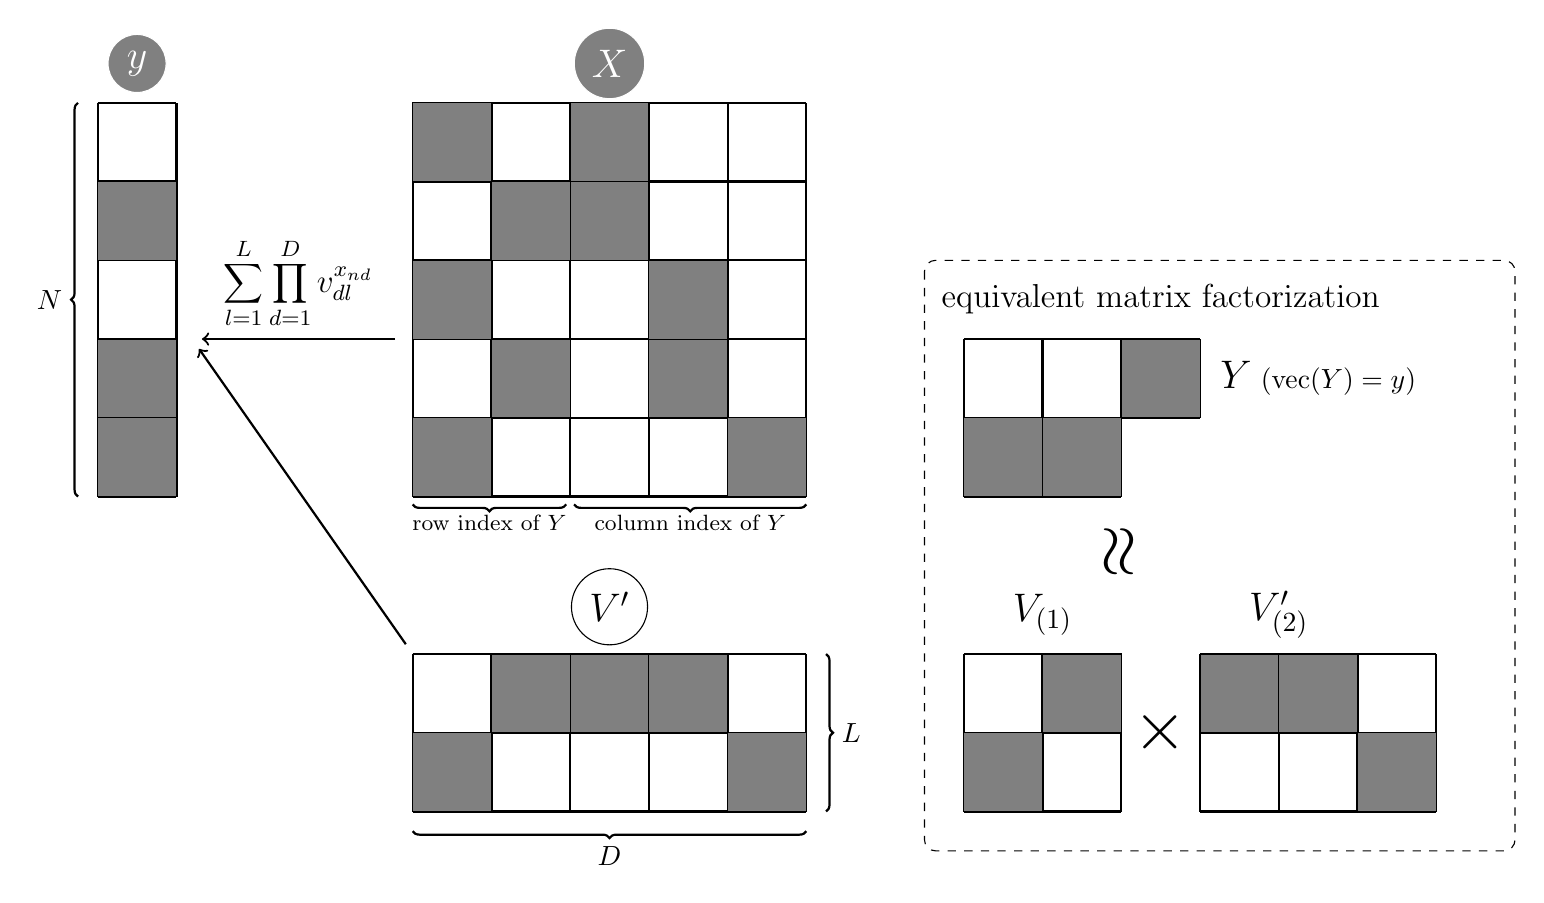
\begin{tikzpicture}
\def\rxo{4}
%brace
\draw [decorate, decoration = {brace}, thick] (-0.25, 0) --  (-0.25, 5) node [midway, left, xshift=-2pt]{$N$}; %y
\draw [decorate, decoration = {brace, mirror}, thick] (\rxo, -4.25) --  (\rxo+5, -4.25) node [midway, below, yshift=-2pt]{$D$}; 
\draw [decorate, decoration = {brace, mirror}, thick] (\rxo+5.25, -4) --  (\rxo+5.25, -2) node [midway, right, xshift=+2pt]{$L$}; %V
%matrix
\draw[step=1cm, black, thick] (1, 5) grid (0,0); %y
\draw[step=1cm, black, thick] (\rxo+5, 5) grid (\rxo,0); %X
\draw[step=1cm, black, thick] (\rxo, -2) grid (\rxo+5, -4); %V

\draw [decorate, decoration = {brace, mirror}, thick] (\rxo, -0.1) --  (\rxo+1.95, -0.1) node [midway, below]{\footnotesize row index of $Y$}; %below X
\draw [decorate, decoration = {brace, mirror}, thick] (\rxo+2.05, -0.1) --  (\rxo+5, -0.1) node [midway, below]{\footnotesize column index of $Y$}; %below X

%label
\node[draw, circle, color=white, fill=gray] (Y) at (0.5, 5.5) {\Large $y$};
\node[draw, circle,  color=white, fill=gray] (X) at (\rxo+2.5, 5.5) {\Large $X$};
\node[draw, circle, black] (V) at (\rxo+2.5, -1.4) {\Large $V'$};
%fill Y
\foreach \x in {0, 1, 3} \draw[fill=gray] (0, \x) rectangle ++(1,1);
% fill X
\foreach \x in {(\rxo, 0), (\rxo,4), (\rxo+1,3), (\rxo, 2), (\rxo+1, 1)} \draw[fill=gray] \x rectangle ++(1,1);
\foreach \x in {(\rxo+4, 0), (\rxo+2,4), (\rxo+2, 3), (\rxo+3,2), (\rxo+3,1)} \draw[fill=gray] \x rectangle ++(1,1);
%fill V
\foreach \x in {(\rxo,-4), (\rxo+1, -3), (\rxo+2,-3), (\rxo+3,-3), (\rxo+4,-4)} \draw[fill=gray] \x rectangle ++(1,1);
%dummy node
\node (dY) at (1.2, 2){};
\node (dX) at (\rxo-0.1, 2){};
\node (dV) at (\rxo, -2){};
\draw[->, thick] (dX)--(dY) node[midway, above]{\large $\displaystyle \sum_{l=1}^{L}\prod_{d=1}^D v_{dl}^{x_{nd}}$};
\draw[->, thick] (dV)--(dY);
%%
%Y matrix
\draw[step=1cm, black, thick] (\rxo+7, 0) grid (\rxo+9,2);
\draw[step=1cm, black, thick] (\rxo+9, 1) grid (\rxo+10,2);
\foreach \x in {0,1} \draw[fill=gray] (\rxo+\x+7, 0) rectangle ++(1,1);
\draw[fill=gray] (\rxo+2+7, 1) rectangle ++(1,1);
%%
%V matrix
\draw[step=1cm, black, thick] (\rxo+7, -2) grid (\rxo+9, -4); %left
\foreach \x in {(\rxo+7,-4), (\rxo+8, -3)} \draw[fill=gray] \x rectangle ++(1,1);
\draw[step=1cm, black, thick] (\rxo+10, -2) grid (\rxo+13, -4); %right
\foreach \x in { (\rxo+10,-3), (\rxo+11,-3), (\rxo+12,-4)} \draw[fill=gray] \x rectangle ++(1,1);
%label (right)
\draw[rounded corners, dashed]  (\rxo+6.5, 3) rectangle (\rxo+14, -4.5);
\node[rotate=90] (app) at (\rxo+9, -0.7){\Huge $\approx$};
\node (times) at (\rxo+9.5, -3){\Huge $\times$};
\node (Ym) at (\rxo+11.5, 1.5) {{\Large $Y$} ($\mathrm{vec}(Y)=y$)};
\node (V) at (\rxo+8, -1.5) {\Large $V_{(1)}$};
\node (V) at (\rxo+11, -1.5) {\Large $V'_{(2)}$};
\node (plate) at (\rxo+9.5, 2.5) {\large equivalent matrix factorization};
\end{tikzpicture}
\end{document}